\chapter{Sicherheitsdienste}\label{Sicherheitsdienste}

In den vorherigen Kapiteln wurden Angriffsmöglichkeiten und die Anforderungen an ein verteiltes System untersucht. In diesem Kapitel erfolgt eine Konkretisierung der Sicherheitsdienste, die
ein verteiltes System bereitstellen muss um als sicher zu gelten. Dieses Kapitel erklärt die unterschiedlichen Dienste und stellt sie anschaulich anhand von Beispielen dar.

\section{Vertraulichkeit}
Die Vertraulichkeit macht Daten nur für eine Gruppe von autorisierten Benutzern verfügbar und schützt sie so vor unbefugten Zugängen. Diese Daten können verschiedene Arten von Informationen,
wie zum Besipiel Nachrichten, Videos oder Filme, Passwörter oder Kontodaten sein. Ein konkretes Beispiel wäre ein Film auf Amazon Prime. Dieser Film ist nur denjenigen
Benutzern verfügbar, die ihn gekauft oder geliehen haben. Um ein weiteres Beispiel handelt es sich bei den Anmeldedaten eines Benutzers. Die Verbindung zwischen Benutzer
und Server muss stets verschlüsselt sein, sodass kein Unbefugter die Anmeldedaten abgreifen kann. \cite{Kriha.2008}
\\\\
In verteilten Systemen funktioniert der Vertraulichkeitsdienst  entweder durch Zugriffsbeschränkungen über einen Kontrollmechanismus oder Verschlüsselung der Informationen (vgl \cite{Mirhakkak.1993}).
Für die Verschlüsselung kann beispielsweise das TLSP Protokoll herangezogen werden. Die Informationen werden vom Protokoll vor dem Senden verschlüsselt und vor dem Empfang wieder entschlüsselt.
So werden die Nachrichten gesichert übermittelt, sind aber dennoch für die Kommunikationspartner zugänglich. Die Vertraulichkeit dient der Sicherstellung des Schutzes der Daten und stellt eine Grundvoraussetzung für erfolgreiche Authentifizierung
und Autorisierung dar. Der Vertraulichkeitsdienst stellt sicher, dass während dem Informationsaustausch keine Manipulationen oder Abfangen der Daten von passiven Angreifern erfolgt ist. \cite{Mirhakkak.1993}
Die Vertraulichkeit dient jedoch nicht nur dem Schutz der Daten vor Unbefugten, sondern trägt auch zur Anonymität der Benutzer bei.
In einem verteilten Informationssytem kann der Vertraulichkeitsdienst Beispielsweise durch Nutzerprofile erfolgen. Hier erhält jeder nur Zugriff auf die ihm zugewiesenen Bereiche. Die persönlichen Daten wie Name und
Adresse sind durch Anmeldename und Kennwort geschützt. Um zu verhindern, dass ein Unbefugter Anmeldename und Passwort abgreifen kann, wird die Verbindung mit einem Sicherheitszertifikat verschlüsselt.


\section{Authentifizierung}

Authentifizierung sogrt dafür, dass ein Benutzer gegenüber einem System verifiziert werden kann.
Der Begriff der Authentifizierung wird oft synonym mit den Begriffen Authentisierung und Autorisierung verwendet. 
Die Authentifizierung lässt sich in weitere Bestandteile untergliedern. Der erste Bestandteil ist die Authentisierung, 
wobei der Benutzer gegenüber dem System eine Identität vorgibt, die von diesem bestätigt werden soll. 
Auf die Authentisierung folgt anschließend die Authentifizierung. Bei dem Authentifizierungsvorgang werden die vom Nutzer 
eingegebenen Daten, also seine angegebene Identität, überprüft. Ist die Überprüfung abgeschlossen folgt die 
Autorisierung. Die Autorisierung ist für die Zuteilung der Zugriffsrechte verantwortlich. 
Durch den Prozess der Authentifizierung wird eine Identität an ein Subjekt/ Entität gebunden. 
Das Binden der Identität berechtigt den Benutzer bestimmte Dienste in Anspruch nehmen zu können. 
\newline
Es gibt verschiedene Arten wie eine Authentifizierung durchgeführt werden kann:
\begin{figure}[H]
    \centering
    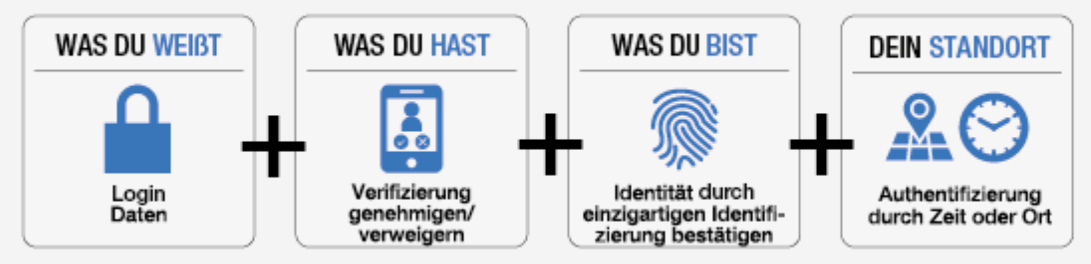
\includegraphics[width=\textwidth]{images/authent_pos1.png}
    \caption[Authentifizierungsarten]{Authentifizierungsarten} 
    \label{Authentifizierungsarten}
\end{figure} 

Im Zusammenhang mit verteilten Systemen im Internet ist die Authentifizierung durch Wissen,
also Benutzername und Passwort, weit verbreitet. 
Das Passwort besteht dabei meistens aus einer Zeichenkombination und wird über einen geschützten Kanal ausgetauscht. 
Besonders bei Diensten im Internet bietet sich die Verwendung von Hyper-Text-Transfer-Protocol-Secure (HTTPS), statt
des ungesicherten Hyper-Text-Transfer-Protocol (HTTP) an.
Das auslesen der Benutzerdaten aus dem Netzwerkverkehr ist so nicht mehr möglich. 
Mit Verwendung eines sicheren Protokolles für die Übermittlung der Daten ist die Übertragung zwischen den Systemen 
als Angriffsvektor ausgeschlossen. 
Sind die Daten erfolgreich und sicher an das Serversystem übermittelt worden müssen diese in bestimmter Form 
(bspw. in einer Datenbank) persistiert werden. 
Das festhalten der Daten im Klartext würde die Datenbank zu einem sehr lohnenden Ziel machen, da die Daten 
an einer stelle gesammelt einsehbar wären. 
Aus diesem Grund benutzt man verschiedene Verschlüsselungsfunktionen um zumindest die Passwörter in eine Form zu bringen,
die nicht wieder re-konstruiert werden kann. Das Anwenden der Verschlüsselungsfunktion wird 
als Hashing bezeichnet. Gehashte Passwörter in der Datenbank bieten eine notwendige Sicherheit um die Daten in sicherer Form 
dauerhaft zu abzulegen. Abgesehen von der Authentifizierung durch Wissen mittels Benutzername und Passwort gibt es die Möglichkeit sich durch 
Besitzt, Identität oder den Standort zu Authentifizieren. 
Besonders interessant für zusätzliche Sicherheit auf Client-Seite können die 
Authentifizierungsmöglichkeiten kombiniert werden. Die Kombination von bspw. einer Authentifizierung durch Wissen und von Besitz 
wird als 2-Faktor-Authentifizierung bezeichnet. Gelangt ein Angreifer an ein Passwort hat er so ohne die entpsrechende zweite 
Authentifizierungsmethode keine Möglichkeit die Identität des Benutzers anzunehmen. 

\section{Integrität}

Das Schutzziel Integrität umfasst sowohl die Korrektheit der Daten (Datenintegrität) 
als auch die korrekte Funktionsweise des Systems (Systemintegrität). 
Es gibt schwache und starke Integrität. 
Eine starke Integrität liegt vor, wenn keine Möglichkeit der unbefugten Datenmanipulation besteht. 
Von einer schwachen Integrität spricht man hingegen dann, falls eine Datenmanipulation zwar generell, 
aber auf keinen Fall unbemerkt möglich ist. 
Mögliche Manipulationen sind z.B. das
Verändern von Daten
Löschen von Daten
Einfügen von Daten
Grundsätzlich ist es fast unmöglich Veränderungen an digitalen Daten vollständig zu vermeiden. 
Dadurch das man die Veränderungen von Daten nicht vermeiden kann, versucht man dem Benutzer die 
Änderung der Daten erkennbar zu machen. 
Besonders im Linux Umfeld hat sich eine überprüfung von Downloads mittels Prüfsummen etabliert.
Zu der eigentlichen Download Dateien ist zusätzlich die Information \glqq SHA265SUM\grqq{ } gegeben (siehe \autoref{Pruefsumme}).
\newline
Es gibt verschiedene Arten wie eine Authentifizierung durchgeführt werden kann:
\begin{figure}[H]
    \centering
    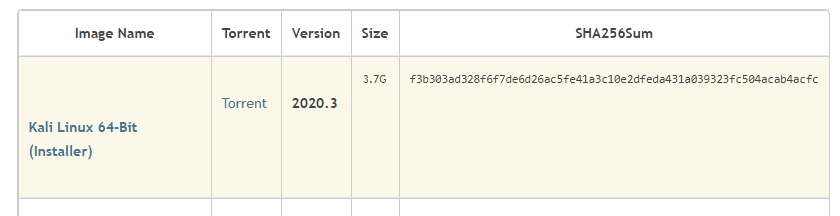
\includegraphics[width=\textwidth]{images/checksum_pic1.png}
    \caption[Prüfsumme]{Pruefsumme} 
    \label{Pruefsumme}
\end{figure}  
Nach dem Download der Datei kann die Prüfsumme über die heruntergeladene Datei erfolgen,
sind die beiden Hashwerte identisch ist der Download valide. 
Stimmen die beiden Prüfsummen nicht über ein, wurde der Download manipuliert und die 
Integrität der Daten wurde verletzt.

\section{Nicht-Anfechtbarkeit}

Das Schutzziel der Nicht-Anfechtbarkeit wurde früher hauptäschlich im Bereich des Informationsaustausches verwendet. Jedem Kommunikationsteilnehmer soll nachgewiesen werden können, welche Informationen er 
versendet oder erhalten hat. Hierfür werden verschiedene Arten der Nachweisbarkeit benötigt. Durch die Nachweisbarkeit der Identität wird das Verleugnen von Nachrichten verhindert und zusätzlich der Betrug verhindert.
Die Nachweisbarkeit des Sendens bezeugt, dass die entsprechenden Informationen auch wirklich gesendet wurden. Ergänzend hierzu kann die Nachweisbarkeit des Zustellens bezeugen, dass der Empfänger die Informationen
auch tatsächlich erhalten hat. \cite{Bedner.2010}
\\\\
Mit dem Zeitalter der Digitalisierung erweiterte sich diese Begriffdefinition auf Handlungen und Transaktionen (vgl \cite{Bedner.2010}).
Unter Nicht-Anfechtbarkeit versteht man heute das Erzeugen eines Nachweises für eine bestimmte Handlung oder Aktion. Der Beweis dient dazu, zu dokumentieren und festzuhalten was ein Benutzer getätigt hat. 
Der Nicht-Anfechtbarkeitsdienst
dient im Streitfall dazu, die erfolgten Aktionen zwischen zwei Kommunikationspartnern Dritten zu beweisen.
Ein konrektes Beispiel wäre ein Überwachungssystem mit Kameras und audiovisueller Aufnahme, wie es Kriha in seinem Buch \cite{Kriha.2008} beschriebt. Um die Daten vor Gericht verwertbar zu machen, muss garantiert werden, dass die Aufnahme von einer der Überwachungskameras stammt.
Weiterhin darf es nciht möglich sein Audiodateien einzuschleusen und so Daten zu fälschen. Auch in Online-Shops in Beriechen des E-Commerce ist Nicht-Anfechtbarkeit wichtig.
Kauft ein Kunde etwas, so muss der Shop genau festhalten was der Kunde gekauft hat. Sind diese Daten nicht-anfechtbar abgespeichert, so kann dem Kunde stets die Inanspruchnahme des zahlungspflichtigen Dienstes
bewiesen werden. Besonders wichtig ist auch wie beim Beispiel des Überwachungssystems die Glaubhaftigkeit des Nachweises, sodass die Möglichkeit der Fälschung von Nachweisen ausgeschlossen werden kann.
Der Nicht-Anfechtbarkeitsdienst sollte aus diesem Grund einen erfolgten Informationsaustausch so dokumentieren, dass der Nachweis nicht gefälscht oder selbst erzeugt sein könnte. 
den Begriff Nicht-Anfechtbarkeit verwendet man auch häufig zusammen mit dem Begriff \glqq Digitale Signatur\grqq{}. Auch die digitale Signatur ist eine Form der Garantie von Nicht-Anfechtbarkeit. 
Es wird die Identität des Benutzers überprüft und ein gültiges Dokument durch eine elektronsiche Unterschrift rechtskräftig unterzeichnet.
\\\\
Es gibt keine konkreten Algorithmen oder Vorgaben, wie der Nicht-Anfechtbarkeitsdienst in verteilten Systemen implementiert werden kann.
Die Implementierung ist stark von der Klasse des verteilten Systems abhängig.

\section{Zugriffssteuerung/Autorisierung}

Nachdem ein sicherer Tunnel durch die Dienste Authentifizierung, Vertraulichkeit und 
Integritätsschutz aufgebaut wurde, befasst sich die Autorisierung mit der Frage wie die Daten 
anschließend verarbeitet werden. 
In Computernetzwerken sowie im Bereich von verteilten Systemen bezeichnet die Autorisierung das Zuweisen 
und die Überprüfung von Zugriffsrechten. Damit bilden Autorisierung und Zugriffssteuerung eine Einheit und 
verantworten die Vergabe von Freigaben an den Benutzer. 
Es gibt verschiedene Arten wie festgelegt werden kann auf welche Ressourcen welcher Benutzer einen Zugriff hat. 
Meist werden die Benutzer zum Stand der Registrierung bereits in eine Benutzergruppe eingeteilt. 
Mithilfe von Gruppenbasierter Zugriffssteuerung können mehrere Rechte mit einem Mal an einen Benutzer übergeben werden. 
Zusätzlich kann mehr Arbeit in die Ganularität der Gruppenberechtigungen investiert werden, als 
wenn für jeden Benutzer eigene Rehte vergeben werden würden. 
Ein Besipiel für eine Gruppenbasierte Zugriffssteuerung ist die Rechtevergabe in Betriebssystemen wie Linux und Windows.
Bei Linux gibt es eine sog. \glqq root\grqq{}-Gruppe, die über Adminsitratorrechte verfügt. Ist ein Benutzerkonto teil dieser Gruppe
kann ohne Einschränkung Software Installiert werden. Ist ein Benutzer in keiner Gruppe muss für die Installation von Software 
das Administrator Kennwort eingegeben werden. 
In verteilten Systemen ist ein ähnliches Prinzip zu beobachten. So gibt es für eine Webanwendung oftmals 
eine Administratorgruppe und Beispielsweise eine Gruppe mit der Bezeichnung \glqq Kunde\grqq{} die nur den Zugriff auf 
einen Teilbereich der Webanwendung zulässt. 

\section{Verfügbarkeit}

Der Sicherheitsdienst Verfügbarkeit garantiert, dass das verteilte System und die angeforderten Daten für seine Benutzer zeitgerecht zur Verfügung steht. Die Datenverarbeitung muss stets ordnungsgemäß
und inhaltlich korrekt sein. \cite{Bedner.2010}
Dieser Dienst wird in den aufgeführten Quellen stets im Rahmen der informationstechnischen Systeme verwendet. Der Verfügbarkeitsdienst
  zielt vorallem darauf ab zu verhindern, 
dass Angreifer über Malware das System ausschalten. Oftmals funktioniert das Auschalten über mehrere kontaminierte Clients, die gleichzeitig auf das System zugreifen. 
Diese Aktion hat eine Überlastung des Ziel-Servers und infolgedessen einen System-Absturz zur Folge. \cite{Kriha.2008}
\newline
Betrachtet man die Dauer der Verfügbarkeit des verteilten Systems im Verhältnis zu der Gesamtzeit, so ist das verteilte System optimalerweise 100\% verfügbar. Dies kann in der Realtiät jedoch kaum erreicht werden.
Fällt ein System aus, so wird die gesamte Ausfallzeit als Downtime bezeichnet. \cite{Bedner.2010}
\newline
 Um die Downtime des Systems möglichst gering zu halten gibt es verschiedene Maßnahmen, die je nach Art des verteilten Systems und auch
dem konkreten Grund des Ausfalls variieren. Als eine sehr allgemine Maßnahme nennt beispielsweise Bedner in seinem Zeitungsartikel \cite{Bedner.2010} die Verwendung redundanter Systeme. Bei einem Ausfall
des Hauptsystems kann das redundante System verwendet werden und ein Absturz wird somit verhidndert. Dies betrifft beispielsweise besonders verteilte Systeme der erneuerbaren Engerien.
Für das konkrete Beispiel eines informationstechnischen Systems schreibt Kriha in seinem Buch \cite{Kriha.2008} über das Besipiel eines Angriffs. Um zu verhindern das kontaminierte Clients das System zu Absturz
bringen, müssen Load-Balancing-Mechanismen verwendet werden. Dies sind Mechanismen, die der Lastverteilung dienen. Ist ein Server überlastet, so leitet er die Anfragen an einen redundant arbeitenden Server weiter.
Eingesetzt wird dies zum Beispiel bei allen großen Streaming Anbietern wie etwa Netflix.
